% ==============================================================================
% Statistical Methods and Site Comparison
% ==============================================================================

\subsection{Statistical Approach}
\label{sec:statistical_methods}

XRF measurements at 3~mm intervals are spatially autocorrelated (lag-1 $r$ = 0.68), so we used core sections as the unit of analysis rather than individual measurements. This yields $n$ = 11 sections at TAM and $n$ = 16 at SC. Site differences were evaluated using Wilcoxon rank-sum tests with Bonferroni correction for multiple comparisons.

\subsection{Site Comparison}
\label{sec:site_comparison}

TAM sediments are consistently more reducing than SC sediments (Figure~\ref{fig:site_comparison}). TAM sections have higher Fe/Mn ratios (median 82 vs.\ 49; $p$ = 0.004) and a greater proportion of reducing conditions (96\% vs.\ 47\% of measurements exceeding Fe/Mn = 50). This difference is robust across all threshold choices tested (Table~\ref{tab:threshold_sensitivity}).

\begin{figure}[h]
\centering
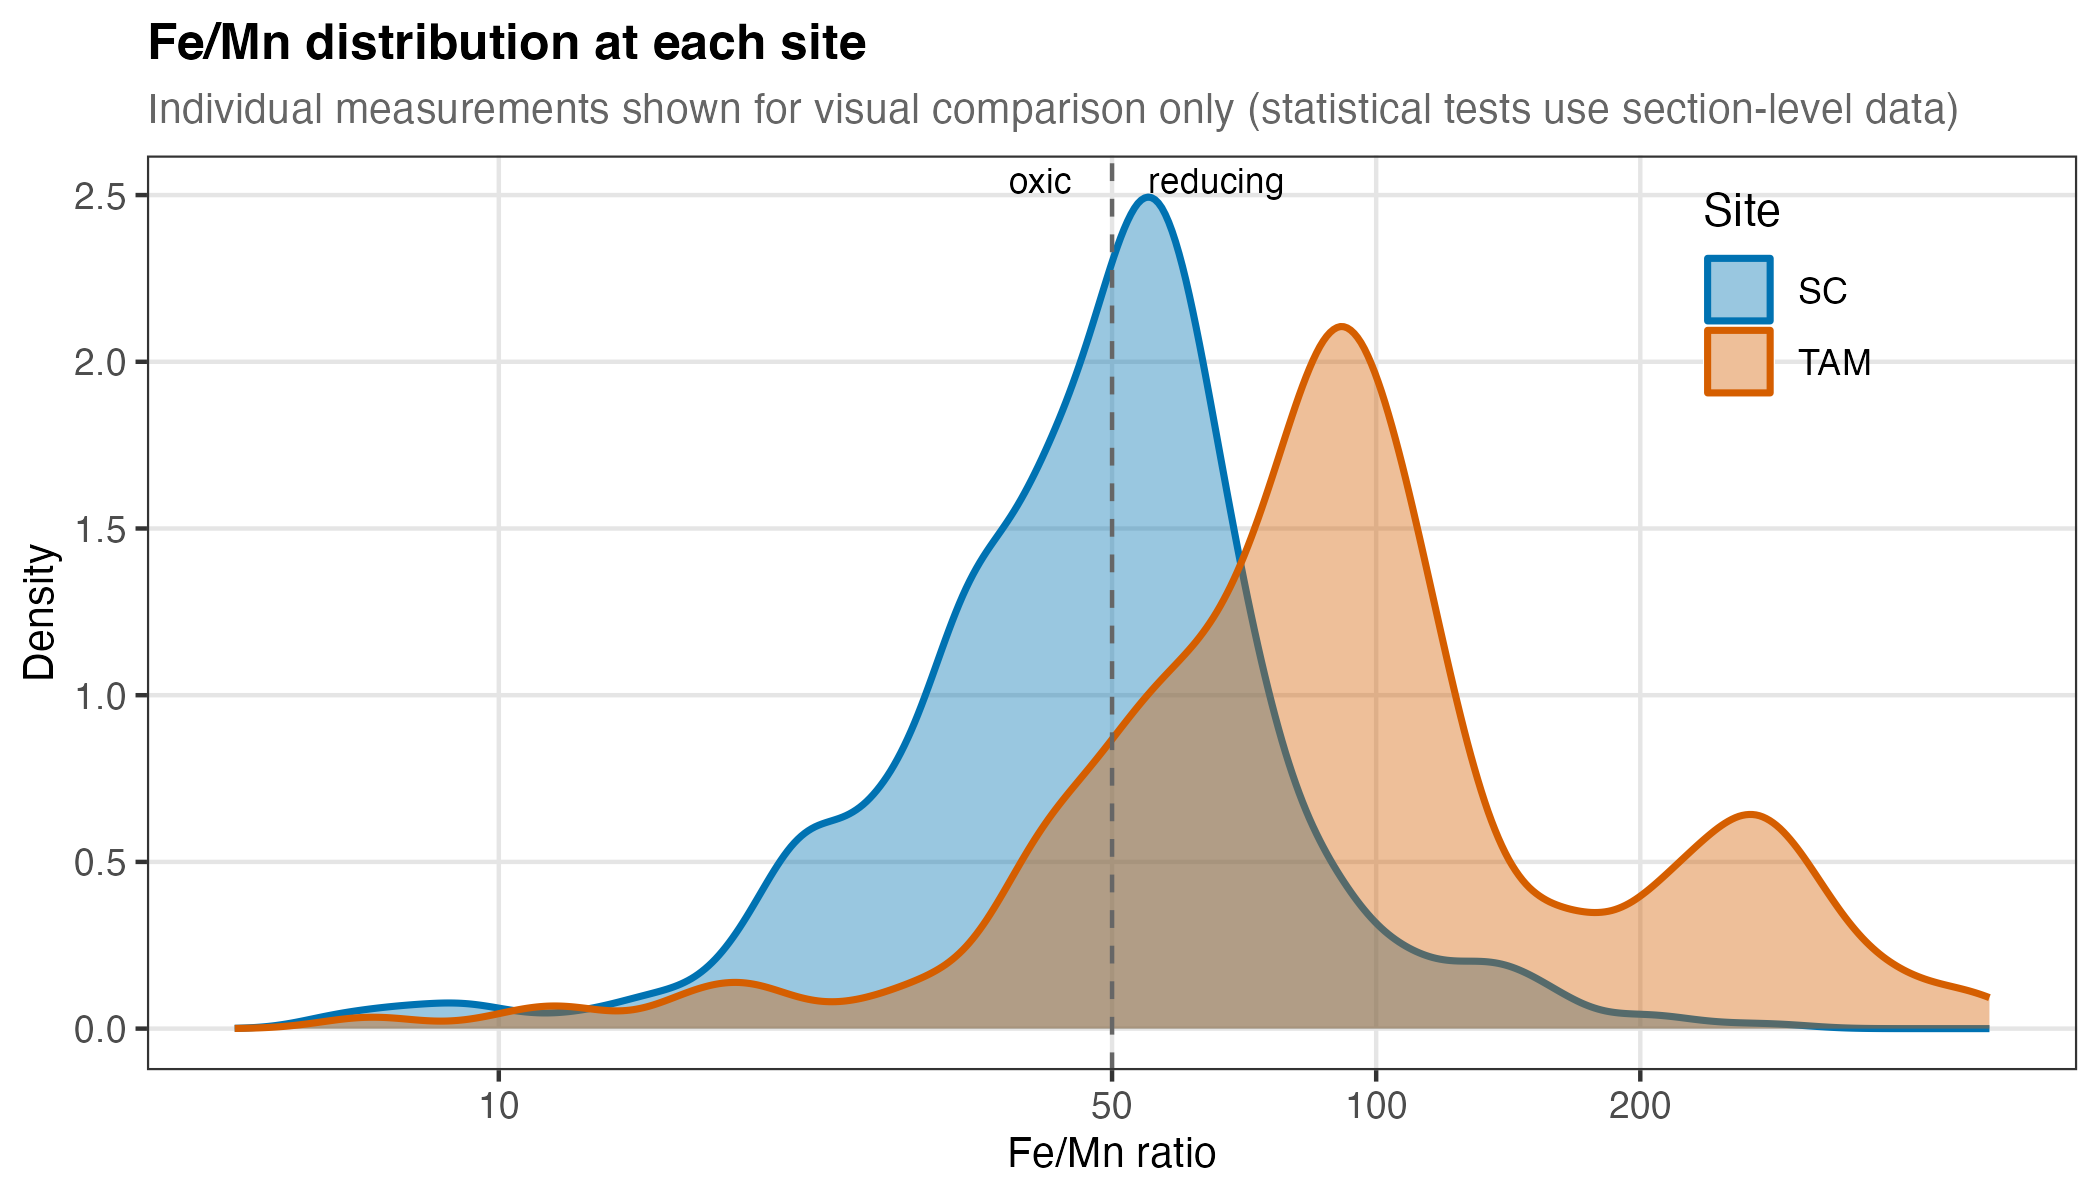
\includegraphics[width=0.7\textwidth]{figures/site_comparison/fig_femn_distribution.png}
\caption{Fe/Mn distribution by site. TAM sediments cluster above the reducing threshold while SC sediments straddle it. Individual measurements shown; statistical tests use section-level data ($n$ = 11 vs 16).}
\label{fig:site_comparison}
\end{figure}

\begin{table}[h]
\centering
\caption{Site difference is robust to threshold choice}
\label{tab:threshold_sensitivity}
\begin{tabular}{rrrr}
\toprule
Fe/Mn threshold & TAM (\%) & SC (\%) & $p$-value \\
\midrule
30 & 94 & 85 & 0.022 \\
50 & 84 & 49 & 0.003 \\
80 & 52 & 7 & $<$0.001 \\
100 & 31 & 4 & 0.002 \\
\bottomrule
\end{tabular}
\end{table}

Other proxies (Ti, Zr/Rb, Ca/Ti) show suggestive but non-significant differences after correction for multiple comparisons (Appendix~\ref{sec:appendix_stats}).

\subsection{Interpretation}
\label{sec:interpretation}

The persistent redox difference between TAM and SC could reflect differences in water depth, organic loading, basin restriction, or diagenetic history. The available data cannot distinguish among these mechanisms, but the magnitude and consistency of the Fe/Mn difference indicates a genuine environmental distinction between the two localities.

% Spectral analysis found no significant periodicities (Appendix~\ref{sec:appendix_spectral}).
